\begin{figure}
  \centering
  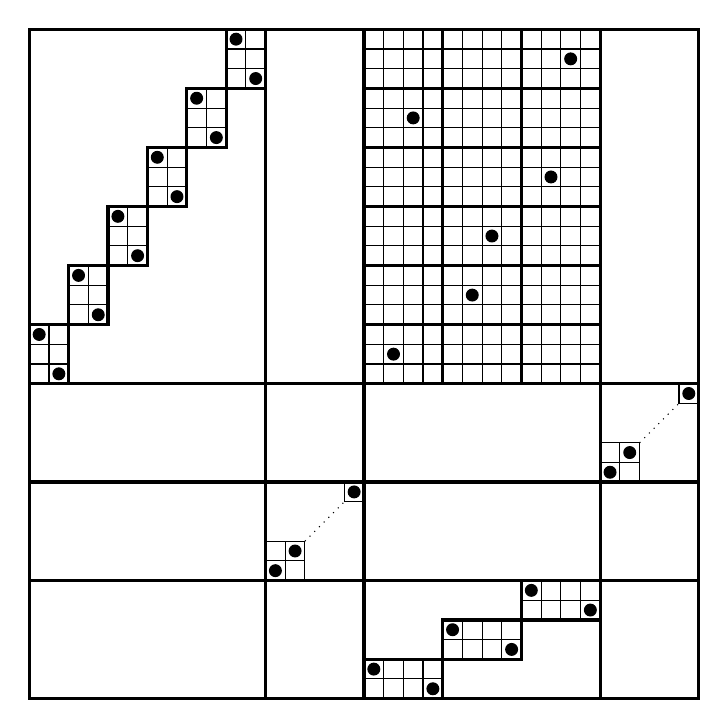
\begin{tikzpicture}
  [
    scale=.25,
  ]
    
    % grid
    \draw [step=1.0, black, very thick] (0,0) rectangle (34,34);
    \draw [step=1.0, black, very thick] (12,0) -- (12,34);
    \draw [step=1.0, black, very thick] (17,0) -- (17,34);
    \draw [step=1.0, black, very thick] (29,0) -- (29,34);
    \draw [step=1.0, black, very thick] (0,6) -- (34,6);
    \draw [step=1.0, black, very thick] (0,16) -- (34,16);
    \draw [step=1.0, black, very thick] (0,11) -- (34,11);

    % vertices
    \def\y{16}
    \foreach \i in {1,2,...,6} {
      \draw [step=1.0, black] (2*\i - 2, \y + 3*\i - 3) grid (2*\i, \y + 3*\i);
      \draw [black, very thick] (2*\i - 2, \y + 3*\i - 3) rectangle (2*\i, \y + 3*\i);
      \draw [fill=black] (2*\i - 1.5, \y + 3*\i - .5) circle (0.3);
      \draw [fill=black] (2*\i - .5, \y - 2 + 3*\i - .5) circle (0.3);
    }
    
    % edges
    \draw [step=1.0, black] (17,16) grid (29, 34);
    \draw [black, very thick] (17,16) rectangle (29, 34);
    \foreach \k/\i/\j in {1/1/5,2/2/3,3/4/6} {
      \draw [step=1.0, black] (4*\k + 13, 2*\k - 2) grid (4*\k + 17, 2*\k);
      \draw [black, very thick] (4*\k + 13, 2*\k - 2) rectangle (4*\k + 17, 2*\k);
      \draw [fill=black] (4*\k + 13 + 1 - .5, 2*\k - .5) circle (0.3);
      \draw [fill=black] (4*\k + 13 + 4 - .5, 2*\k - 1 - .5) circle (0.3);
      \draw [fill=black] (4*\k + 13 + 2 - .5, 16 + 3*\i - 1 - .5) circle (0.3);
      \draw [fill=black] (4*\k + 13 + 3 - .5, 16 + 3*\j - 1 - .5) circle (0.3);
    }
    % vertical
    \draw [black, very thick] (21, 16) -- (21, 34);
    \draw [black, very thick] (25, 16) -- (25, 34);
    % horizontal
    \draw [black, very thick] (17, 19) -- (29, 19);
    \draw [black, very thick] (17, 22) -- (29, 22);
    \draw [black, very thick] (17, 25) -- (29, 25);
    \draw [black, very thick] (17, 28) -- (29, 28); 
    \draw [black, very thick] (17, 31) -- (29, 31);

    % separators 2
    \def\x{29}
    \def\y{11}
    \def\i{1}
    \def\xs2{\x + 5*\i - 5}
    \def\ys2{\y - 5*\i + 5}
    \draw [black, very thick] (\xs2, \ys2) rectangle (\xs2 + 5, \ys2 + 5);
    \draw [step=1.0, black] (\xs2, \ys2) grid (\xs2 + 2, \ys2 + 2);
    \draw [dotted] (\xs2 + 2, \ys2 + 2) -- (\xs2 + 4, \ys2 + 4);
    \draw [black] (\xs2 + 4, \ys2 + 4) rectangle (\xs2 + 5, \ys2 + 5);
    \draw [fill=black] (\xs2 + .5, \ys2 + .5) circle (0.3);
    \draw [fill=black] (\xs2 + 1.5, \ys2 + 1.5) circle (0.3);
    \draw [fill=black] (\xs2 + 4.5, \ys2 + 4.5) circle (0.3);

    % separators 1
    \def\x{12}
    \def\y{6}
    \def\i{1}
    \def\xs2{\x + 5*\i - 5}
    \def\ys2{\y - 5*\i + 5}
    \draw [black, very thick] (\xs2, \ys2) rectangle (\xs2 + 5, \ys2 + 5);
    \draw [step=1.0, black] (\xs2, \ys2) grid (\xs2 + 2, \ys2 + 2);
    \draw [dotted] (\xs2 + 2, \ys2 + 2) -- (\xs2 + 4, \ys2 + 4);
    \draw [black] (\xs2 + 4, \ys2 + 4) rectangle (\xs2 + 5, \ys2 + 5);
    \draw [fill=black] (\xs2 + .5, \ys2 + .5) circle (0.3);
    \draw [fill=black] (\xs2 + 1.5, \ys2 + 1.5) circle (0.3);
    \draw [fill=black] (\xs2 + 4.5, \ys2 + 4.5) circle (0.3);
  \end{tikzpicture}

  \caption{\label{fig:example-merge-permutation-pi1}
  Transforming the matching \raisebox{-.25cm}{\EXAMPLEM} into the permutation $\pi^i$, $i \neq 0$..
}% end caption
\end{figure}